\documentclass{beamer}

\mode<presentation>
{
  \usetheme{boxes}

  \usecolortheme{dove}



  \setbeamercovered{transparent}
  % or whatever (possibly just delete it)
}


\usepackage[english]{babel}
% or whatever

\usepackage[latin1]{inputenc}
% or whatever

\usepackage{times}
\usepackage[T1]{fontenc}
% Or whatever. Note that the encoding and the font should match. If T1
% does not look nice, try deleting the line with the fontenc.

\title[Fullstack Javascript Web Applications]{Fullstack Javascript Web Applications}
\author[Chris Gradwohl]{}
\institute[University of California, Santa Cruz]{} % (optional, but mostly needed)

% - Use the \inst command only if there are several affiliations.
% - Keep it simple, no one is interested in your street address.

\date[March 2017]{}
\begin{document}

\begin{frame}
  \titlepage
  \begin{center}
  		Chris Gradwohl \

		University of California, Santa Cruz
  \end{center}
\end{frame}




\begin{frame}{Introduction to Javascript}{}
    % - A title should summarize the slide in an understandable fashion
    %   for anyone how does not follow everything on the slide itself.

    \begin{itemize}
	    \item Stack Overflow has ranked Javascript as the worlds most popular programming language(four years in a row).

		\vspace{2em}

	    \item The language for client side web development.
		\vspace{2em}
	    \item Node.js has made fullstack(client side AND server side) applications possible.
		\vspace{2em}
	\end{itemize}
\end{frame}


\begin{frame}{Introduction to Javascript}{}
	
\includegraphics[width=\textwidth]{write_all_the_code_in_javascript1.jpg}
\end{frame}


\begin{frame}{Introduction to Javascript}{}
	\begin{center}
		
\includegraphics[width=200px, height=200px]{59809489.jpg}
	\end{center}
\end{frame}

\begin{frame}{Why Javascript?}{}
	\begin{itemize}
		\item It's convenient for developers
		\vspace{3em}
		\pause
		\item But more importantly...javascript is a single threaded,
		non-blocking, asynchronous, concurrent language.
	\end{itemize}
\end{frame}

\begin{frame}{Javascript is single threaded}{}
	\begin{itemize}
		\item one thread == one call stack == one thing at a time.
		\pause
		\vspace{2em}
		\item the call stack records where we are in the program.
		\vspace{2em}
		\pause

		\item calling a function means we .push() it onto the stack.
		\vspace{2em}
		\pause

		\item returning from a function means we .pop() it off the stack.
		\vspace{2em}
	\end{itemize}
\end{frame}


\begin{frame}{Blocking and the call stack}{}
	\begin{itemize}
		\item Blocking refers to HOW we .push() functions onto the call stack.
		\vspace{1em}
		\item Synchronous function calls are the problem.
		\vspace{2em}
		\begin{center}
			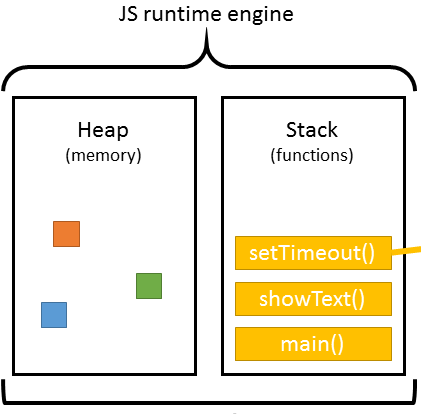
\includegraphics[width=130px, height=130px]{js_runtime.png}
		\end{center}
	\end{itemize}
\end{frame}

\begin{frame}{Blocking and the call stack}{Javascript event loop solves blocking}
	\begin{itemize}
		\item the javascript event loop makes javascript asynchronous and concurrent!
		\vspace{2em}
		\item .push() a function onto the stack
		\vspace{1em}
		\item .pop() the function off the call stack
		\item process functions in the event loop
		\pause
		\item the stack is now free to execute remaining function calls.
		\vspace{2em}
		\pause
		\item callback/return the function when its ready to execute 

	\end{itemize}
\end{frame}


\begin{frame}
	\begin{center}
		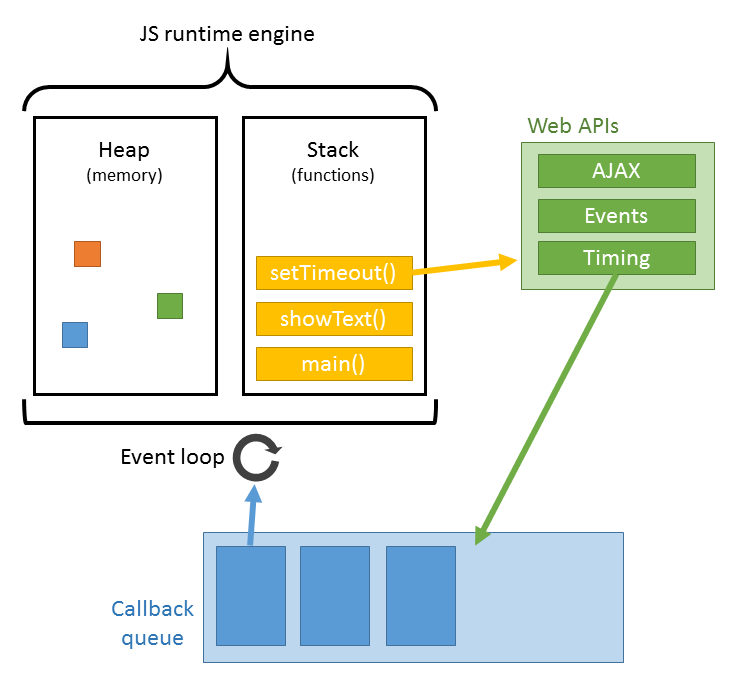
\includegraphics[width=230px, height=230px]{js_runtime2.png}
	\end{center}
\end{frame}


\begin{frame}{Javascript Recap}{}
	\begin{itemize}
		\item Single threaded AND Non-Blocking
		\pause
		\begin{itemize}
			\item one stack == one thing at a time(kind of)
			\pause
			\item there is no downtime, works starts right away
			\pause
			\item made possible by the asynchronous and concurrent event loop.
			\pause
		\end{itemize}
		\item Benefits
		\pause
		\begin{itemize}
			\item fast, no downtime between function calls
			\pause
			\item easier to program versus multithreaded programming
			\pause
			\item less resources: memory, time
		\end{itemize}
	\end{itemize}
\end{frame}

\begin{frame}{Memory Usage}
	\begin{center}
		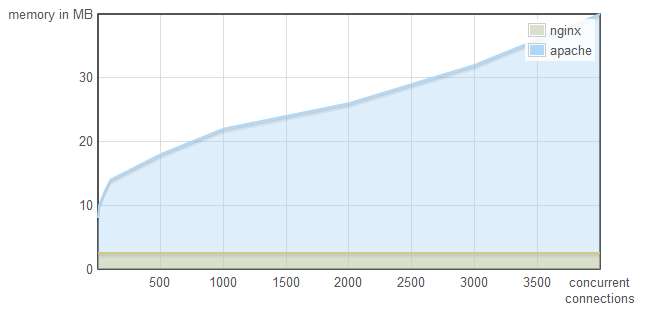
\includegraphics[width=230px, height=230px]{nginx-apache-memory.png}
	\end{center}
\end{frame}

\begin{frame}{Speed}
	\begin{center}
		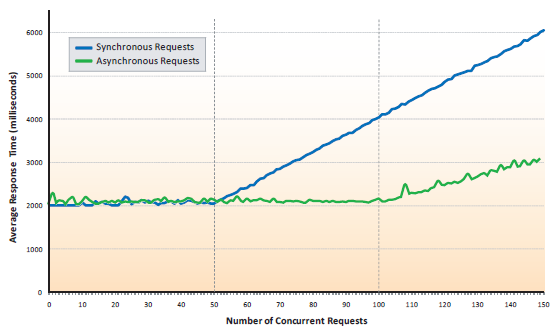
\includegraphics[width=230px, height=230px]{image.png}
	\end{center}
\end{frame}

\begin{frame}{Conclusions}{}
	\begin{itemize}
		\item Javascript is FAST: single threaded, non blocking, asynchronous, and concurrent
		\vspace{2em}
		\item Technologies like Node.js allows developers to use Javascript outside the
		the browser, and inside the server.
		\vspace{2em}
		\item Using javascript on the server, is fast and scalable.
		\vspace{2em}
		\item Allows developers to program both the front-end and backend.
	\end{itemize}
\end{frame}


\begin{frame}{References}

  	\begin{thebibliography}{10}

  	\bibitem{Author1}
    	Saba Alimadadi, Ali Mesbah, Karthik Pattabiraman.
    	\newblock  Understanding Asynchronous Interactions in Full-Stack JavaScript.
		\newblock {\em ICSE '16, May 14 - 22, 2016, Austin, TX, USA}


  	\bibitem{web1}
  		Prashant Bansal.
    	\newblock{\em http://prashantb.me/javascript-call-stack-event-loop-and-callbacks/}


	\bibitem{web2}
    	Steven Sanderson.
      	\newblock{\em http://blog.stevensanderson.com/2010/01/25/measuring-the-performance-of-asynchronous-controllers/}


	\bibitem{web3}
	Stack Overflow.
	\newblock{\em https://stackoverflow.com/research/developer-survey-2016}

  \end{thebibliography}
\end{frame}


\end{document}
